\documentclass[12pt,letter]{article}
\usepackage{geometry}\geometry{top=0.75in}
\usepackage{amsmath}
\usepackage{amssymb}
\usepackage{mathtools}
\usepackage{xcolor} % Color words
\usepackage{cancel} % Crossing parts of equations out
\usepackage{tikz}       % Drawing 
\usetikzlibrary{shapes.geometric, arrows}
\usepackage{pgfplots}   % Other plotting
\usepgfplotslibrary{colormaps,fillbetween}
\usepackage{placeins}   % Float barrier
\usepackage{listings}
\usepackage{enumitem}

\DeclarePairedDelimiter{\ceil}{\lceil}{\rceil}

% Don't indent
\setlength{\parindent}{0pt}
% Function to replace \section with a problem name specifically formatted
\newcommand{\problem}[1]{\vspace{3mm}\Large\textbf{{Problem
{#1}\vspace{3mm}}}\normalsize\\}
% Formatting function, like \problem
\newcommand{\ppart}[1]{\vspace{2mm}\large\textbf{\\Part
{#1})\vspace{2mm}}\normalsize\\}
% Formatting 
\newcommand{\condition}[1]{\vspace{1mm}\textbf{{#1}:}\normalsize\\}

\begin{document}
\title{CIS 510: Project 4G}
\author{Steven Walton}
\maketitle

\section{Introduction} It is disputed which solver to use to solve partial
differential equations (PDE). Two common contenders are the Euler method and
Runge-Kutta 4th (RK4) order method. 

Both methods are Lie Group Integrators, meaning that they are best suited for
functions that are smooth and continuous within the integration domain. We will
not be investigating other solvers.

\subsection{Euler}
The Euler solver is a first order and simple to implement PDE solver. Simply
put, Euler solves by taking an initial position and adding a weighted evaluation
of the function at that point. More rigorously,

\begin{equation}\label{eq:euler}
    y_n = y_{n-1} + hf(t_{n-1}, y_{n-1})
\end{equation}

This is an iterative method that depends on the step-size, $h$, and how many
times we want to iterate. Intuitively, making $h$ smaller results in a more
accurate solution. But if we make $h$ smaller, then we will need to take more
steps. Looking at equation~\ref{eq:euler} we can see that our complexity is
constant times how long it takes to evaluate the function $f$ (assumed to be
constant), we will get a constant complexity. Therefore, while iterating our
complexity will be equal to the number of steps, $N$, that we take, or $O(N)$.

\subsubsection{Advantages}
Euler's method has two distinct advantages: It is easy to implement and it has
low time complexity.

\subsubsection{Disadvantages}
Euler's main downfall is that it is a first order solver, meaning that it has an
error $O(h^1)$.

\subsection{Runge-Kutta}
Runge-Kutta is another common PDE solver. It is a generalized solver, but we
will only be looking at the fourth-order method. RK4 can be solved by using a
weighted summation to the initial value

\begin{equation}\label{eq:rk4}
\begin{split}
    &y = y_{n-1} + h\sum_{i=1}^{4}b_ik_i \\ 
    &k_1 = hf(t_{n-1},y_{n-1}) \\
    &k_2 = hf(t_{n-1} + \frac{h}{2}, y_{n-1} + \frac{k_1}{2}) \\
    &k_3 = hf(t_{n-1} + \frac{h}{2}, y_{n-1} + \frac{k_2}{2}) \\
    &k_4 = hf(t_{n-1} + h, y_{n-1} + k_3) \\
    &\text{generally} \\
    &k_i = f(t_{n-1} + c_ih, y_{n-1} + h(b_{i1}k_1 + \cdots + b_{i,i-1}k_{i-1}))
\end{split}
\end{equation}
We use Simpson's Rule to find all the $b_i$'s. This gives us 

\begin{equation}
    y_n = y_{n-1} + \frac{k_1 + 2k_2 + 2k_3 + k_4}{6}
\end{equation}

Paying attention, we may notice that $k_1$ is equivalent to Euler's method, and
thus we can say that this equation has at more operations and will take longer
to solve than Euler's method. 

The difference here is that RK4 is a fourth-order method, having an accumulation
error of ($O(h^4)$).

\subsubsection{Advantages}
RK4 has one simple advantage: it is a high order method, meaning that it
produces little error. A not so simple advantage is that the algorithm is
extendable, and if we implement a generalized version then we can vary the
accumulation error as our customers see fit.
\subsubsection{Disadvantages}
The disadvantages of RK4 is that it is much more complex, compared to Euler, and
that for a given time-step it takes longer to compute than Euler.

\section{Study}
To understand the differences we'll look at a few different simulations. We
compare Euler and RK4 by 3 different criteria: size of h, number of steps, and
time to solve. We will run several simulations and vary the parameters. The
output is below in Figure~\ref{fig:compare}.

\FloatBarrier
\begin{figure}[ht]
    \label{fig:compare}
    \begin{center}
    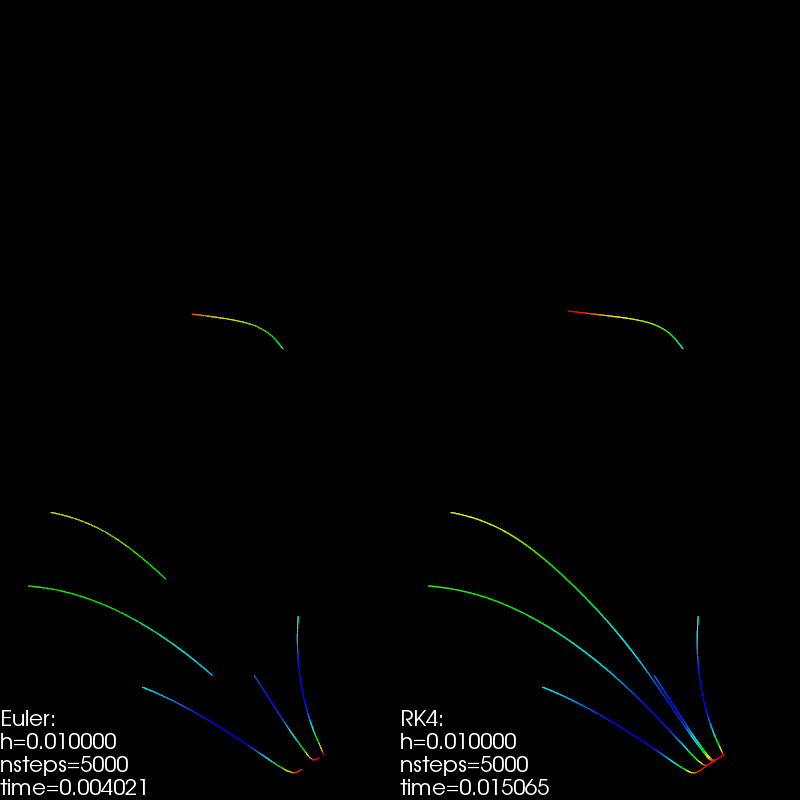
\includegraphics[width=0.24\textwidth]{imgs/h0p01.png}
    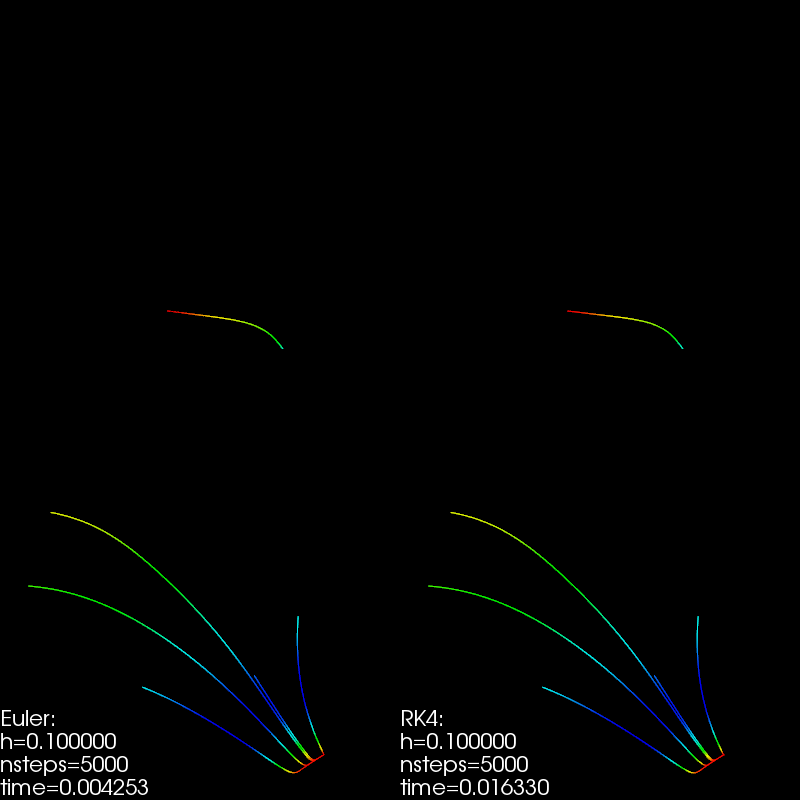
\includegraphics[width=0.24\textwidth]{imgs/h0p1.png}
    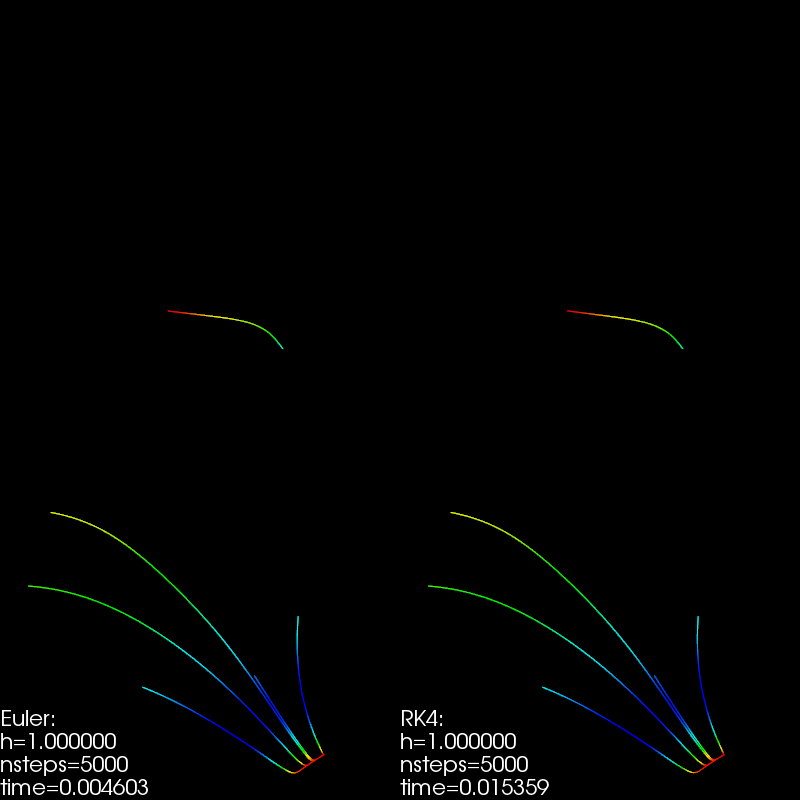
\includegraphics[width=0.24\textwidth]{imgs/h1p0.png}
    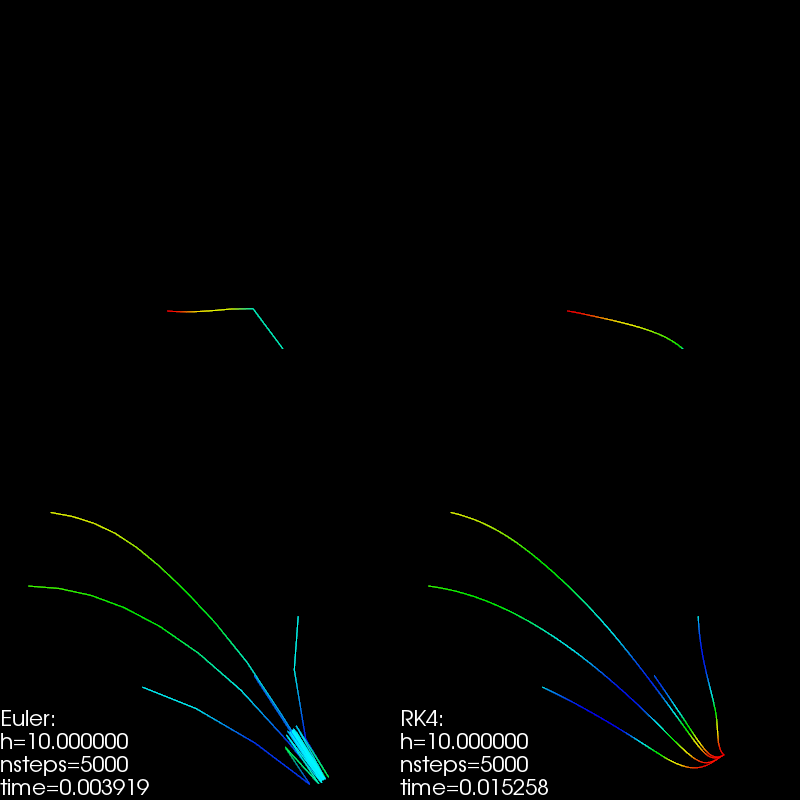
\includegraphics[width=0.24\textwidth]{imgs/h10p0.png}
    %\end{center}
    \\
    %\begin{center}
    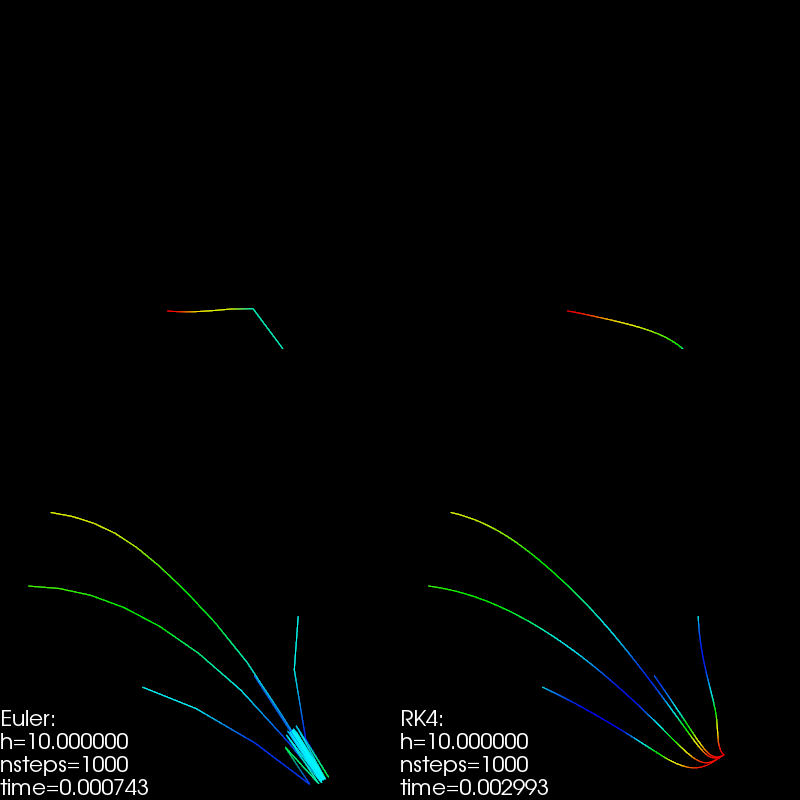
\includegraphics[width=0.24\textwidth]{imgs/h10n1000.png}
    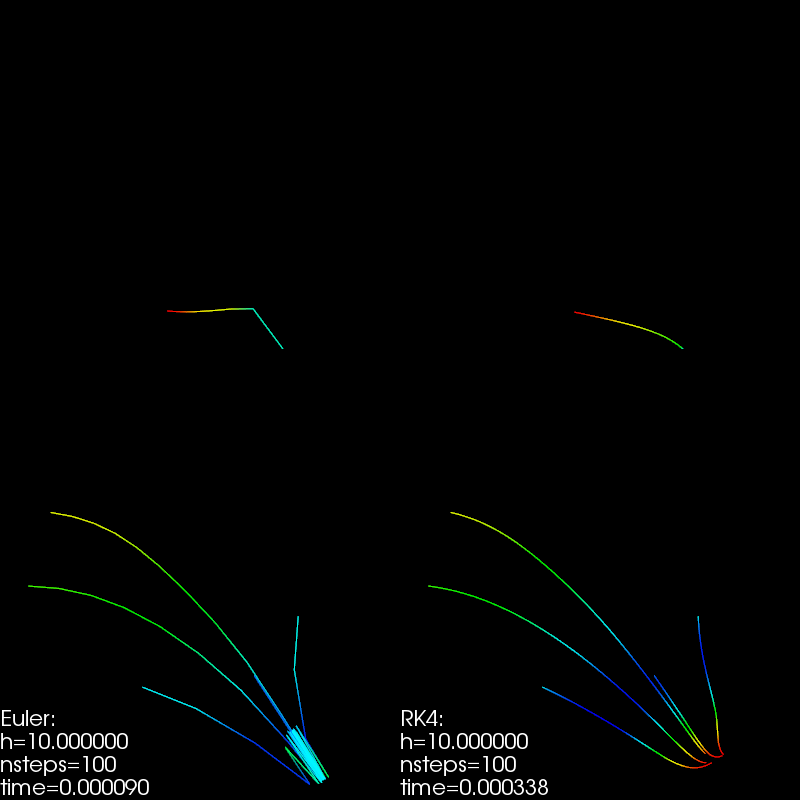
\includegraphics[width=0.24\textwidth]{imgs/h10n100.png}
    \end{center}
    \caption{Row 1: h=\{0.01, 0.1, 1.0, 10.0\} with nsteps=5000. Row 2: h=1.0 and h=\{1000,100\}}
\end{figure}
\FloatBarrier

In the top left image we have Euler with a converged(ish) solution solved in
0.004 seconds. In the bottom right, we have a converged RK4 solution solved in
0.0003 seconds. So from that alone, we have a 10x speedup that RK4 can provide
by taking bigger step sizes ($h$) and solving for a smaller number of steps. If
we pay attention even more, we can tell that the bottom right RK4 solution gives 
us more information that the top left Euler. This shows us that this can be
optimized even further. (We should be a little careful with this analysis, as
neither method is highly optimized and a simplified approach was used for
implementation.)

\section{Conclusion} 

Time is money. That is what it comes down to. Our customers pay for their
compute time, and by saving our customers over 10x in compute time we can better
attract them if our service implements a faster PDE solver. But science is more
nuanced than that. Because of this I recommend that we implement a generalized
Runge-Kutta method. By implementing this we can scale error to the needs of the
customer (RK1 is equivalent to Euler), thus also extending our customer base.  I
recommend that the default solver be set to RK4, as our experiments have shown
that many times this method will be faster for our customers. A default value to
a balance of speed and accuracy simplifies the process for our users and
defaults them to a solution that wins in the majority of cases. This will
generally save our customers money, time, and maximize flexibility.

\end{document}
